\documentclass[border=3pt]{standalone}
% Preâmbulo compartilhado pelos diagramas TikZ da aula 7 de IHR (Emoção)
\usepackage[T1]{fontenc}
\usepackage[utf8]{inputenc}
\usepackage{lmodern}
\usepackage{amsmath}
\usepackage{xcolor}
\usepackage{tikz}
\usetikzlibrary{arrows.meta,angles,quotes,decorations.pathmorphing,decorations.pathreplacing,calc,
                positioning,shapes.geometric,shapes.misc,backgrounds,fit,
                math}

% Paleta (mesma dos SVGs originais)
% Paleta da disciplina de IHR: acento azul (#1A6FB5), cor de destaque do tema.
% (o nome "dblue" é mantido para não alterar todos os diagramas)
\definecolor{dblue}{HTML}{1A6FB5}
\definecolor{dorange}{HTML}{B3541E}
\definecolor{dgreen}{HTML}{4A7C59}
\definecolor{dred}{HTML}{9C4B4B}
\definecolor{dcream}{HTML}{F4F1EA}
\definecolor{dshade}{HTML}{DDD7C9}

% Função gaussiana (não normalizada por padrão de escala visual)
\pgfmathdeclarefunction{gauss}{3}{%
  \pgfmathparse{1/(#3*sqrt(2*pi))*exp(-((#1-#2)^2)/(2*#3^2))}%
}

% Estilos comuns (prefixo d... para não colidir com chaves internas do pgf)
\tikzset{
  >={Stealth[length=2mm]},
  dguide/.style={gray!55, dashed, line width=0.4pt},
  daxis/.style={gray!60, line width=0.7pt, ->},
  dbody/.style={fill=black!3, draw=black!80, line width=1pt},
  dacc/.style={draw=dblue, line width=1pt},
  dlbl/.style={black!55, font=\small},
  dsub/.style={black!45, font=\footnotesize},
  dstate/.style={circle, draw=black!80, fill=dcream, line width=1pt,
                 minimum size=17mm, font=\large, inner sep=1pt},
  dobs/.style={circle, draw=black!80, fill=dshade, line width=1pt,
               minimum size=14mm, font=\large, inner sep=1pt},
  dbox/.style={rounded corners=2pt, draw=black!80, fill=dcream, line width=1pt,
               align=center, inner sep=6pt},
  dop/.style={circle, draw=black!80, fill=white, line width=1pt,
              minimum size=6mm, inner sep=0pt, font=\small},
  dtrans/.style={->, dblue, line width=1pt},
  dmeas/.style={->, dorange, line width=1pt},
  dcurve/.style={line width=1pt, dblue},
  dcurveb/.style={line width=1.4pt, dorange},
}

\begin{document}
\hyphenpenalty=10000 \exhyphenpenalty=10000 \tolerance=9999 \emergencystretch=3em
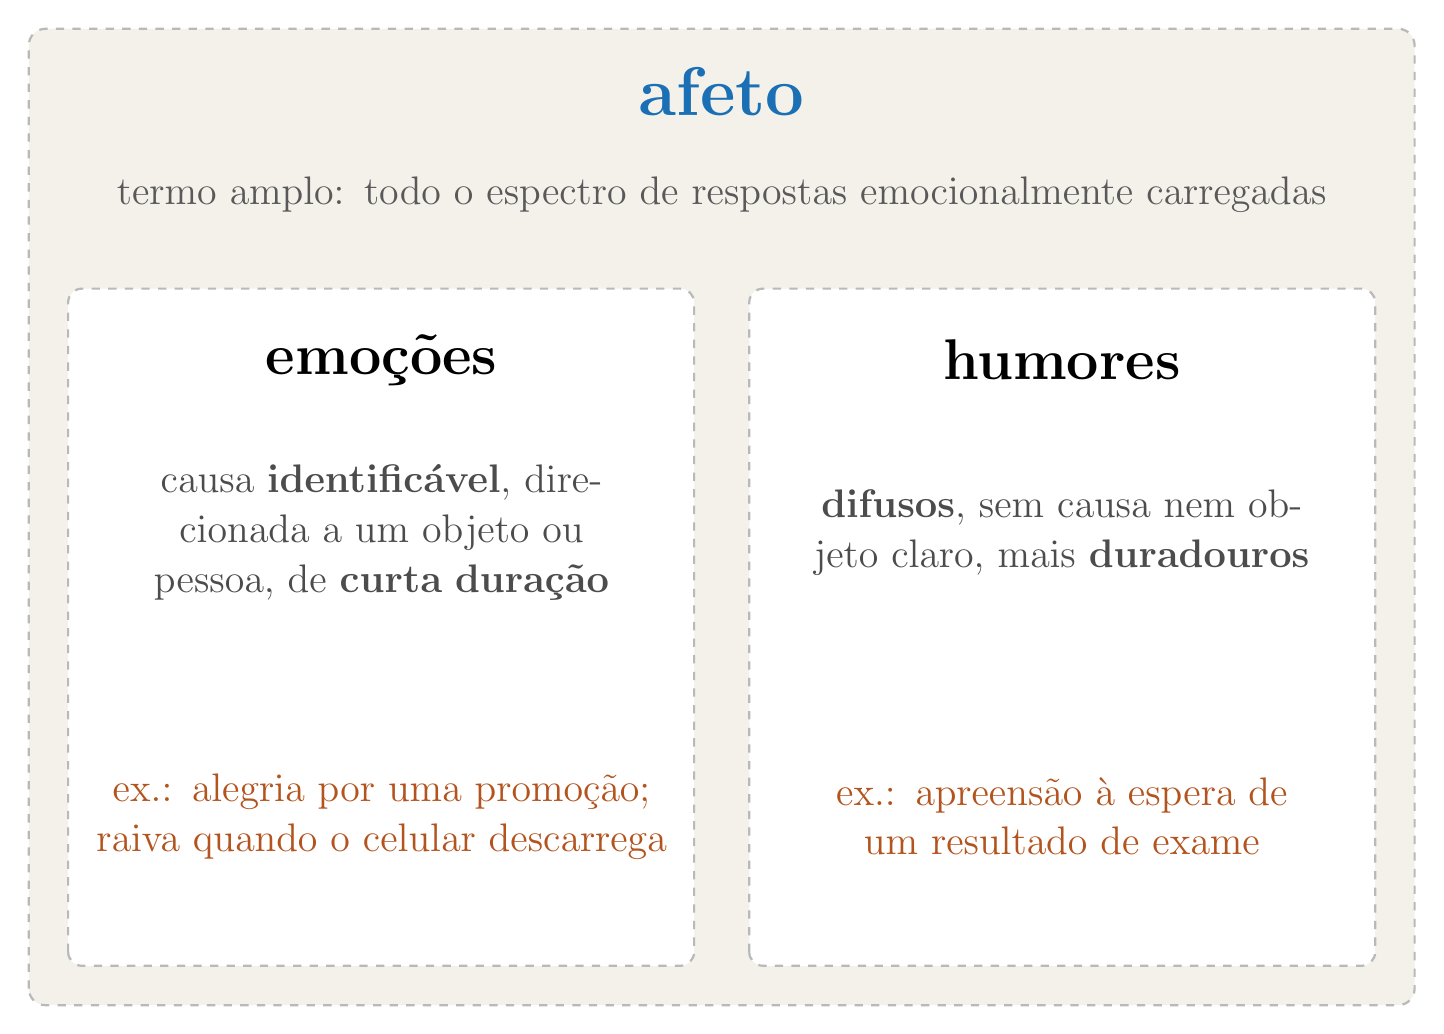
\begin{tikzpicture}[x=1cm,y=1cm]

  \draw[dguide, rounded corners=6pt, fill=dcream, line width=0.8pt] (-8.8,-6.6) rectangle (8.8,5.8);
  \node[font=\Huge\bfseries, dblue] at (0,5.0) {afeto};
  \node[font=\Large, black!65, align=center, text width=15.6cm] at (0,3.7) {termo amplo: todo o espectro de respostas emocionalmente carregadas};

  \draw[dguide, rounded corners=5pt, fill=white, line width=0.8pt] (-8.3,-6.1) rectangle (-0.35,2.5);
  \node[font=\huge\bfseries] at (-4.32,1.6) {emoções};
  \node[font=\Large, black!70, align=center, text width=7.3cm] at (-4.32,-0.6)
     {causa \textbf{identificável}, direcionada a um objeto ou pessoa, de \textbf{curta duração}};
  \node[font=\Large, dorange, align=center, text width=7.3cm] at (-4.32,-4.2)
     {ex.: alegria por uma promoção; raiva quando o celular descarrega};

  \draw[dguide, rounded corners=5pt, fill=white, line width=0.8pt] (0.35,-6.1) rectangle (8.3,2.5);
  \node[font=\huge\bfseries] at (4.32,1.6) {humores};
  \node[font=\Large, black!70, align=center, text width=7.3cm] at (4.32,-0.6)
     {\textbf{difusos}, sem causa nem objeto claro, mais \textbf{duradouros}};
  \node[font=\Large, dorange, align=center, text width=7.3cm] at (4.32,-4.2)
     {ex.: apreensão à espera de um resultado de exame};

\end{tikzpicture}
\end{document}
